%
% lin1.tex
%
% (c) 2018 Prof Dr Andreas Müller, Hochschule Rapperswil
%
\documentclass[tikz]{standalone}
\usepackage{times}
\usepackage{amsmath}
\usepackage{txfonts}
\usepackage[utf8]{inputenc}
\usepackage{graphics}
\usetikzlibrary{arrows,intersections}
\begin{document}

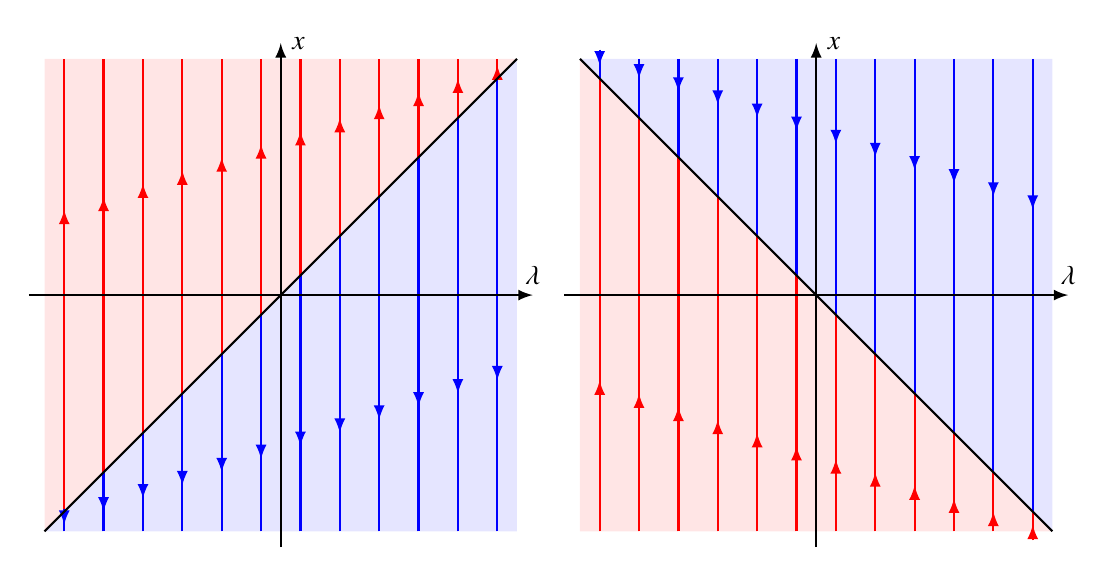
\begin{tikzpicture}[>=latex,thick]

\def\l{3}

\fill[color=red!10] ({-\l},{-\l})--({\l},{\l})--({-\l},{\l})--cycle;
\fill[color=blue!10] ({-\l},{-\l})--({\l},{-\l})--({\l},{\l})--cycle;

\pgfmathparse{-\l+0.25}
\edef\lfirst{\pgfmathresult}
\pgfmathparse{-\l+0.75}
\edef\lsecond{\pgfmathresult}
\pgfmathparse{\l-0.25}
\edef\llast{\pgfmathresult}

\foreach \x in {\lfirst,\lsecond,...,\llast}{
        \draw[color=red] ({\x},{(\x+2*\l)/3-0.2})--({\x},{\l});
        \draw[->,color=red] ({\x,\x})--({\x},{(\x+2*\l)/3});
        \draw[color=blue] ({\x},{-\l})--({\x},{(\x-2*\l)/3+0.2});
        \draw[->,color=blue] ({\x},{\x})--({\x},{(\x-2*\l)/3});
}

\draw ({-\l},{-\l})--({\l},{\l});

\draw[->] ({-\l-0.2},0)--({\l+0.2},0) coordinate[label=$\lambda$];
\draw[->] (0,{-\l-0.2})--(0,{\l+0.2}) coordinate[label={right:$x$}];

\begin{scope}[xshift = 6.8cm]

\fill[color=red!10] ({-\l},{-\l})--({\l},{-\l})--({-\l},{\l})--cycle;
\fill[color=blue!10] ({-\l},{\l})--({\l},{-\l})--({\l},{\l})--cycle;

\foreach \x in {\lfirst,\lsecond,...,\llast}{
        \draw[->,color=red] ({\x},{-\l})--({\x},{(-\x-2*\l)/3});
        \draw[color=red] ({\x},{(-\x-2*\l)/3-0.2})--({\x},{-\x});
        \draw[->,color=blue] ({\x},{\l})--({\x},{(-\x+2*\l)/3});
        \draw[color=blue] ({\x},{(-\x+2*\l)/3+0.2})--({\x},{-\x});
}

\draw ({-\l},{\l})--({\l},{-\l});

\draw[->] ({-\l-0.2},0)--({\l+0.2},0) coordinate[label=$\lambda$];
\draw[->] (0,{-\l-0.2})--(0,{\l+0.2}) coordinate[label={right:$x$}];
\end{scope}

\end{tikzpicture}

\end{document}
